\documentclass[twoside,a4paper]{article}
\usepackage{geometry}
\geometry{margin=1.5cm, vmargin={0pt,1cm}}
\setlength{\topmargin}{-1cm}
\setlength{\paperheight}{29.7cm}
\setlength{\textheight}{25.3cm}

% useful packages.
\usepackage{amsfonts}
\usepackage{amsmath}
\usepackage{amssymb}
\usepackage{amsthm}
\usepackage{enumerate}
\usepackage{graphicx}
\usepackage{multicol}
\usepackage{fancyhdr}
\usepackage{layout}
\usepackage{listings}
\usepackage{float, caption}

\lstset{
    basicstyle=\ttfamily, basewidth=0.5em
}

% some common command
\newcommand{\dif}{\mathrm{d}}
\newcommand{\avg}[1]{\left\langle #1 \right\rangle}
\newcommand{\difFrac}[2]{\frac{\dif #1}{\dif #2}}
\newcommand{\pdfFrac}[2]{\frac{\partial #1}{\partial #2}}
\newcommand{\OFL}{\mathrm{OFL}}
\newcommand{\UFL}{\mathrm{UFL}}
\newcommand{\fl}{\mathrm{fl}}
\newcommand{\op}{\odot}
\newcommand{\Eabs}{E_{\mathrm{abs}}}
\newcommand{\Erel}{E_{\mathrm{rel}}}

\begin{document}

\pagestyle{fancy}
\fancyhead{}
\lhead{Wenchong Huang (3200100006)}
\chead{Numerical PDE homework \#3}
\rhead{Apr.18th, 2023}


\section*{I. Exercise 11.9 (Verify the operator norm.)}

\;\;\;\; Firstly, the set $\mathcal{M}(T)=\{M\geq 0:\forall \mathbf{x}\in \mathbb{F}^n, ||T\mathbf{x}||\leq M||\mathbf{x}||\}$ clearly has a lower bound $0$. Hence by the completeness of $\mathbb{R}$, the infimum indeed exsists.

Now we verify three properties of a norm: positive-definite, positive-homogeneous, and triangle inquality.

If $T=\mathbf{0}$, clearly $||T||=0$. Now suppose that $||T||=0$. Then $\forall \mathbf{x}\in\mathbb{F}^n$, we have $||T\mathbf{x}||\leq ||T||\cdot||\mathbf{x}||=0$. By the positive-definition of vector norm, we have $T\mathbf{x}=0$. By the arbitariness of $\mathbf{x}$, we have $T=0$.

The positive-homogeneity follows immediately by $T(\lambda\mathbf{x})=\lambda T(\mathbf{x})$.

Now for the triangle inequality, We have:
\begin{equation*}
    ||(T+S)\mathbf{x}||=||T\mathbf{x}+S\mathbf{x}||\leq ||T\mathbf{x}||+||S\mathbf{x}|| \leq (||T||+||S||)\cdot ||\mathbf{x}||,\quad \forall\mathbf{x}\in\mathbb{F}^n.
\end{equation*}

Hence $||T||+||S||\in\mathcal{M}(T+S)$, and hence $||T+S||=\inf \mathcal{M}(T+S)\leq ||T||+||S||$.

\section*{II. Exercise 11.3 (Verify d(T,S)=||T-S|| induced a metric space.)}

\;\;\;\; Clearly we have:
\begin{itemize}
    \item non-negativity: $d(T,S)=||T-S||\geq 0$,
    \item positive-definition: $d(T,S)=0 \iff T-S=\mathbf{0} \iff T=S$,
    \item symmetry: $d(T,S)=||T-S||=||S-T||=d(S,T)$.
\end{itemize}

Now by the triangle inequality of operator norm, we have:
\begin{equation*}
    d(T,S)+d(S,P) = ||T-S|| + ||S-P|| \geq ||T-S+S-P||=||T-P||=d(T,P).
\end{equation*}

Hence $d(T,S)$ is indeed a distence, and hence induced a metric space.

\section*{III. Exercise 11.16 (Verify the Hilbert-Schmidt norm.)}

\;\;\;\; The positive-definition and the positive-homogeneity are trivial. Now let's verify the triangle inequality.
\begin{align*}
    |T+S|^2 &= \sum_{j=1}^n ||T\mathbf{e}_j+S\mathbf{e}_j||^2\\
    &= \sum_{j=1}^n ||T\mathbf{e}_j||^2+||S\mathbf{e}_j||^2+2\langle T\mathbf{e}_j,S\mathbf{e}_j \rangle\\
    &= |T|^2 + |S|^2 + 2\sum_{j=1}^n\langle T\mathbf{e}_j,S\mathbf{e}_j \rangle\\
    &\leq |T|^2 + |S|^2 + 2\sqrt{\sum_{j=1}^n ||T\mathbf{e}_j||^2||S\mathbf{e}_j||^2}\\
    &\leq |T|^2 + |S|^2 + 2\sqrt{\sum_{j=1}^n ||T\mathbf{e}_j||^2\sum_{i=1}^n||S\mathbf{e}_i||^2}\\
    &=|T|^2 + |S|^2 + 2\sqrt{|T|^2|S|^2}\\
    &=|T|^2 + |S|^2 + 2|T|\cdot|S| =(|T|+|S|)^2.
\end{align*}

Hence $|T+S|\leq |T|+|S|$, where the forth step below follows from the Cauchy inequality.

\section*{IV. Exercise 11.20 (Prove $|TS|\leq |T||S|$)}

\;\;\;\; By corollary 11.18 we know $||T\mathbf{x}||\leq |T|\cdot ||\mathbf{x}||$, hence
\begin{equation*}
    |TS|^2=\sum_{j=1}^n||TS\mathbf{e}_j||^2\leq \sum_{j=1}^n|T|^2\cdot ||S\mathbf{e}_j||^2=|T|^2\sum_{j=1}^n ||S\mathbf{e}_j||^2=|T|^2|S|^2.
\end{equation*}

\section*{V. Exercise 11.36 (Prove $\text{det}(e^X)=e^{\text{tr} X}$)}

\;\;\;\; By Jordan decomposition theorem, $\forall X\in\mathbb{R}^{n\times n}\;\text{or}\;\mathbb{C}^{n\times n}$, we have
\begin{equation*}
    X=P^{-1}JP,
\end{equation*}

where $P$ is orthogonal and $J=\text{diag}(J_1,...,J_k)$ is the Jordan canonical form of $X$. $J_i\;(i=1,...,k)$ is Jordan block of size $m_i$, where
\begin{equation*}
    J_i=\begin{bmatrix}
        \lambda_i & 1\\
        & \lambda_i & 1\\
        & & \ddots & \ddots\\
        & & & \lambda_i & 1\\
        & & & & \lambda_i
    \end{bmatrix}.
\end{equation*}

Clearly we have:
\begin{equation*}
    J_i^n = \begin{bmatrix}
        \lambda_i^n & * & * & \cdots & *\\
        & \lambda_i^n & * & \cdots & *\\
        & & \ddots & \ddots & \vdots\\
        & & & \lambda_i^n & *\\
        & & & & \lambda_i^n
    \end{bmatrix},\qquad \forall n\in\mathbb{Z}_+,
\end{equation*}

where '*' means an element that we don't care about. And hence
\begin{equation*}
    e^{J_i} = \begin{bmatrix}
        \sum_{n=0}^\infty \frac{\lambda_i^n}{n!} & * & * & \cdots & *\\
        & \sum_{n=0}^\infty \frac{\lambda_i^n}{n!} & * & \cdots & *\\
        & & \ddots & \ddots & \vdots\\
        & & & \sum_{n=0}^\infty \frac{\lambda_i^n}{n!} & *\\
        & & & & \sum_{n=0}^\infty \frac{\lambda_i^n}{n!}
    \end{bmatrix}=\begin{bmatrix}
        e^{\lambda_i} & * & * & \cdots & *\\
        & e^{\lambda_i} & * & \cdots & *\\
        & & \ddots & \ddots & \vdots\\
        & & & e^{\lambda_i} & *\\
        & & & & e^{\lambda_i}
    \end{bmatrix}.
\end{equation*}

Note that $e^{J_i}$ is an upper triangle matrix, we can immediately get the determinant:
\begin{equation*}
    \text{det}(e^{J_i})=\left(e^{\lambda_i}\right)^{n_i}=e^{n_i\lambda_i}.
\end{equation*}

By lemma 11.32 we have $e^{P_{-1}JP}=P^{-1}e^J P$, hence 
\begin{equation*}
    \text{det}(e^X)=\text{det}(P^{-1} e^J P)=\text{det}(e^J).
\end{equation*}

We could easily verify that for any block diagonal matrix $A=\text{diag}(A_1,...,A_k)$, we have:
\begin{equation*}
    e^A=\text{diag}(e^{A_1},...,e^{A_k}).
\end{equation*}

And hence
\begin{equation*}
    \text{det}(e^J)=\text{det} (\text{diag}(e^{J_1},...,e^{J_k})) = \prod_{i=1}^k \text{det}(e^{J_i})=\prod_{i=1}^k e^{n_i\lambda_i}=e^{\sum_{i=1}^k n_i\lambda_i}.
\end{equation*}

Use a well-know conclution in lineaer algebra: $\text{tr}\;A$ is equal to the sum of all eigenvalues of $A$ (containing multiple eigenvalues). We proved that
\begin{equation*}
    \text{det}(e^X)=e^{\sum_{i=1}^k n_i\lambda_i}=e^{\text{tr}\;X}.
\end{equation*}

\section*{VI. Exercise 11.50 (Prove the solution of IVP is not overly seneitive to the initial condition)}

\;\;\;\; If $\mathbf{v_0}=\mathbf{w_0}$, then the conclution is trivial. Now we suppose $\mathbf{v_0}>\mathbf{w_0}$. Let $G(t)=\mathbf{v}(t-a)-\mathbf{w}(t-a)$, we assert that $G(t)\geq 0$. Otherwise let
\begin{equation*}
    t^* = \sup\{t>0:\forall 0\leq s\leq t, G(s)\geq 0\}.
\end{equation*}

By the continuity of $G$ and $G(0)>0$, also by the assumption that $\exists x\;\text{s.t.}\; G(x)<0$, we konw $t^*$ indeed exsists. And clearly $G(t^*)=0$, hence $\mathbf{v}(t^*)=\mathbf{w}(t^*)$. Then let $\hat{v}$ be the solution of
\begin{equation*}
    \left\{\begin{array}{l}
        \frac{\text{d} \hat{v}}{\text{d}t}=f(\hat{v}(t),t+t^*),\\
        \hat{v}(0)=\mathbf{v}(t^*).
    \end{array}\right.
\end{equation*}

Clearly $\mathbf{v}(t)=\hat{v}(t-t^*)$ and $\mathbf{w}(t)=\hat{v}(t-t^*)$ for any $t>t^*$. By the uniqueness of $\hat{v}$, we have $\mathbf{v}(t)=\mathbf{w}(t)$ for any $v\geq t^*$. That's a contradiction.

Now we proved $G(t)\;(t\geq 0)$ is a non-negative function which satisfies
\begin{equation*}
    G'(t) = f(\mathbf{v}(t),t)-f(\mathbf{w}(t),t) \leq L(\mathbf{v}(t)-\mathbf{w}(t))=LG(t),\quad \forall t\geq 0.
\end{equation*}

Hence by Gronwall's inequality, we have
\begin{equation*}
    G(t)\leq e^{Lt}G(0).
\end{equation*}

And hence
\begin{equation*}
    |\mathbf{v}(t)-\mathbf{w}(t)|=\mathbf{v}(t)-\mathbf{w}(t)=G(t-a)\leq e^{L(t-a)}|\mathbf{v}_0-\mathbf{w}_0|.
\end{equation*}

Similar for $\mathbf{v_0}<\mathbf{w_0}$.

\section*{VII. Exercise 11.100 (Compute the first five coefficients $C_j$)}

\;\;\;\; For the trapezoidal method, we have
\begin{equation*}
    s=1,\;\alpha_1=1,\;\alpha_0=-1,\;\beta_1=\beta_0=\frac{1}{2}.
\end{equation*}

Hence
\begin{align*}
    C_0 &= \alpha_0+\alpha_1=0\\
    C_1 &= -\beta_0+\alpha_1-\beta_1=0\\
    C_2 &= \frac{1}{2}\alpha_1-\beta_1=0\\
    C_3 &= \frac{1}{6}\alpha_1-\frac{1}{2}\beta_1=-\frac{1}{12}\\
    C_4 &= \frac{1}{24}\alpha_1-\frac{1}{6}\beta_1=-\frac{1}{24}.
\end{align*}

For the midpoint rule, we have
\begin{equation*}
    s=2,\;\alpha_2=1,\;\alpha_1=0,\;\alpha_0=-1,\;\beta_1=2,\;\beta_0=0.
\end{equation*}

Hence
\begin{align*}
    C_0 &= \alpha_0+\alpha_1+\alpha_2=0\\
    C_1 &= -\beta_0+\alpha_1-\beta_1+2\alpha_2=0\\
    C_2 &= \frac{1}{2}\alpha_1-\beta_1+2\alpha_2=0\\
    C_3 &= \frac{1}{6}\alpha_1-\frac{1}{2}\beta_1+\frac{4}{3}\alpha_2=\frac{1}{3}\\
    C_4 &= \frac{1}{24}\alpha_1-\frac{1}{6}\beta_1+\frac{2}{3}\alpha_2=\frac{1}{3}.
\end{align*}

\section*{VIII. Exercise 11.102 (Express conditions of $||\mathcal{L}\mathbf{u}(t_n)||=O(k^3)$)}

\;\;\;\; By lemma 11.95, to achieve $O(k^3)$ accuracy, we must have $C_0=C_1=C_2=0$, i.e.
\begin{equation*}
    \sum_{j=0}^s \alpha_j=0,\qquad \sum_{j=0}^s j\alpha_j=\sum_{j=0}^s \beta_j,\qquad \sum_{j=0}^sj^2\alpha_j=2\sum_{j=0}^sj\beta_j,
\end{equation*}

which is equivalanet to
\begin{equation*}
    \rho(1)=0,\qquad \rho'(1)=\sigma(1),\qquad \rho'(1)+\rho''(1)=\frac{1}{2}\sigma'(1).
\end{equation*}

\section*{IX. Exercise 11.103 (Derive coefficients of LMMs)}

\;\;\;\; Use c++, do symbolic computation with my \verb|fracMatrix|, \verb|fraction| and \verb|bigint| library. The code is here.

\begin{lstlisting}
    #include "matrix_fraction.h"
    #include <bits/stdc++.h>
    using namespace std;
    
    void Adams_Bashforth(){
        cout << "-----------------------Adams Bashforth-----------------------" << endl;
        for(int s = 1; s <= 5; s++){
            cout << "s=" << s << "  p=" << s << "  ";
            fraction a[s+1];
            a[s] = 1;
            a[s-1] = -1;
            fracMatrix coef(s,s);
            fracMatrix rhs(s,1);
            for(int q = 1; q <= s; q++){
                for(int j = 0; j < s; j++){
                    coef.element(q-1,j) = fraction(bigPow(j,q-1), bigFact(q-1));
                    rhs.element(q-1,0) += fraction(bigPow(j,q), bigFact(q)) * a[j];
                }
                rhs.element(q-1,0) += fraction(bigPow(s,q), bigFact(q)) * a[s];
            }
            fracMatrix b = solve(coef, rhs);
            cout << b.reverse().T();
        }
    }
    
    void Adams_Moulton(){
        cout << "------------------------Adams Moulton------------------------" << endl;
        for(int s = 1; s <= 5; s++){
            cout << "s=" << s << "  p=" << s+1 << "  ";
            fraction a[s+1];
            a[s] = 1;
            a[s-1] = -1;
            fracMatrix coef(s+1,s+1);
            fracMatrix rhs(s+1,1);
            for(int q = 1; q <= s+1; q++){
                for(int j = 0; j <= s; j++){
                    coef.element(q-1,j) = fraction(bigPow(j,q-1), bigFact(q-1));
                    rhs.element(q-1,0) += fraction(bigPow(j,q), bigFact(q)) * a[j];
                }
            }
            fracMatrix b = solve(coef, rhs);
            cout << b.reverse().T();
        }
    }
    
    void BDF(){
        cout << "--------------Backward Differentiation Formula---------------" << endl;
        for(int s = 1; s <= 5; s++){
            cout << "s=" << s << "  p=" << s << "  ";
            fracMatrix coef(s+2,s+2);
            fracMatrix rhs = zeros(s+2,1);
            for(int q = 0; q <= s; q++){
                for(int j = 0; j <= s; j++){
                    coef.element(q,j+1) = fraction(bigPow(j,q), bigFact(q));
                }
                if(q >= 1) coef.element(q,0) = -fraction(bigPow(s,q-1), bigFact(q-1));
            }
            coef.element(s+1,s+1) = 1;
            rhs.element(s+1,0) = 1;
            fracMatrix ab = solve(coef, rhs);
            cout << ab.reverse().T();
        }
    }
    
    int main(){
        Adams_Bashforth();
        Adams_Moulton();
        BDF();
        return 0;
    }
\end{lstlisting}

You can goto the folder \verb|src| and compile the code by:
\begin{lstlisting}
    g++ ex11-103.cpp -o ex -O2
\end{lstlisting}

And run it by:
\begin{lstlisting}
    ./ex
\end{lstlisting}

The running result is here. We computed one more formula than the textbook.

\begin{lstlisting}
    -----------------------Adams Bashforth-----------------------
    s=1  p=1  [ 1 ]
    s=2  p=2  [ 3/2, -1/2 ]
    s=3  p=3  [ 23/12, -4/3, 5/12 ]
    s=4  p=4  [ 55/24, -59/24, 37/24, -3/8 ]
    s=5  p=5  [ 1901/720, -1387/360, 109/30, -637/360, 251/720 ]
    ------------------------Adams Moulton------------------------
    s=1  p=2  [ 1/2, 1/2 ]
    s=2  p=3  [ 5/12, 2/3, -1/12 ]
    s=3  p=4  [ 3/8, 19/24, -5/24, 1/24 ]
    s=4  p=5  [ 251/720, 323/360, -11/30, 53/360, -19/720 ]
    s=5  p=6  [ 95/288, 1427/1440, -133/240, 241/720, -173/1440, 3/160 ]
    --------------Backward Differentiation Formula---------------
    s=1  p=1  [ 1, -1, 1 ]
    s=2  p=2  [ 1, -4/3, 1/3, 2/3 ]
    s=3  p=3  [ 1, -18/11, 9/11, -2/11, 6/11 ]
    s=4  p=4  [ 1, -48/25, 36/25, -16/25, 3/25, 12/25 ]
    s=5  p=5  [ 1, -300/137, 300/137, -200/137, 75/137, -12/137, 60/137 ]    
\end{lstlisting}

\section*{X. Exercise 11.108 (Verify the accuracy of 3-order BDF)}

\;\;\;\; We need to show that
\begin{equation*}
    \lim_{z\to 1} \frac{\frac{\rho(z)}{\sigma(z)}-\log z}{(z-1)^4}=C\neq 0.
\end{equation*}

By exercise 11.103, we have known that
\begin{equation*}
    \rho(z)=-\frac{2}{11}+\frac{9}{11}z-\frac{18}{11}z^2+z^3,\quad \sigma(z)=\frac{6}{11}z^3.
\end{equation*}

Use th\'eorem de L'h\^opital, we got
\begin{align*}
    \lim_{z\to 1} \frac{\frac{\rho(z)}{\sigma(z)}-\log z}{(z-1)^4} &= \lim_{z\to 1} \frac{-\frac{1}{3}z^{-3}+\frac{3}{2}z^{-2}-3z^{-1}+\frac{11}{6}-\log z}{(z-1)^4}= \lim_{z\to 1}\frac{z^{-4}-3z^{-3}+3z^{-2}-z^{-1}}{4(z-1)^3}\\
    &= \lim_{z\to 1}\frac{-4z^{-5}+9z^{-4}-6z^{-3}+z^{-2}}{12(z-1)^2} = \lim_{z\to 1}\frac{20z^{-6}-36z^{-5}+18z^{-4}-2z^{-3}}{24(z-1)}\\
    &=\lim_{z\to 1}\frac{-120z^{-7}+180z^{-6}-72z^{-5}+6z^{-4}}{24}=-\frac{1}{4}\neq 0.
\end{align*}

\section*{XI. Exercise 11.109}

\;\;\;\; Prove the necessity first. Suppose that an $s$-step LMM has order of accuracy $p$. By lemma 11.95 we have:
\begin{equation*}
    \mathcal{L}\mathbf{u}(t_n)=\sum_{n=0}^\infty C_nk^n\frac{\text{d}^n \mathbf{u}}{\text{d} t^n} (t_n)
\end{equation*}

Since it has order of accuracy $p$, by definition 11.96 we have $C_0=C_1=\cdots =C_p=0$. If $\mathbf{u}_t$ is a polynomial of degree $<p$, then $\frac{\text{d}^n \mathbf{u}}{\text{d} t^n}\equiv 0$ for any $n\geq q+1$. Hence $\mathcal{L}\mathbf{u}\equiv 0$. However for $\mathbf{u}_t$ of degree $p$, $\mathcal{L}\mathbf{u}=C_{q+1}k^{q+1}\frac{\text{d}^{q+1} \mathbf{u}}{\text{d} t^{q+1}}\not\equiv 0.$

Now prove the sufficiency. Apply induction to prove $C_0=\cdots =C_p=0$, and finally prove $C_{p+1}\neq 0$. Take $\mathbf{u}(t)=c\in\mathbb{C}$, then $\mathbf{u}_t$ is polynomial of degree $<p$, hence
\begin{equation*}
    \mathcal{L}\mathbf{u}\equiv 0\implies C_0c=0\;(\forall c\in\mathbb{C}) \implies C_0=0.
\end{equation*}

Now suppose we have proved $C_0=\cdots=C_{m-1}=0$ for some $m\leq p$. Take $\mathbf{u}(t)=\frac{ct^m}{m!},\;c\in\mathbb{C}$, then $\mathbf{u}_t$ is polynomial of degree $<p$, hence
\begin{equation*}
    \mathcal{L}\mathbf{u}=C_mk^m\frac{\text{d}^m \mathbf{u}}{\text{d} t^m}\equiv 0\implies C_mk^mc=0\;(\forall c\in\mathbb{C}) \implies C_m=0.
\end{equation*}

Hence we proved $C_0=C_1=\cdots =C_p=0$ by induction. Now take $\mathbf{u}(t)=\frac{t^{p+1}}{(p+1)!}$, then $\mathbf{u}_t$ is polynomial of degree $p$, hence
\begin{equation*}
    \mathcal{L}\mathbf{u}=C_{p+1}k^{p+1}\frac{\text{d}^{p+1} \mathbf{u}}{\text{d} t^{p+1}}\not\equiv 0\implies C_{p+1}k^{p+1}\neq 0 \implies C_{p+1}\neq 0.
\end{equation*}

Hence by the definition, the LMM has order of accuracy $p$.

\section*{XII. Exercise 11.113 (Compute the characteristic polynomial of $M$)}

\;\;\;\; Compute the determinant by the following steps:
\begin{align*}
    p_M(z)=\text{det}(zI-M)&=\text{det}\begin{bmatrix}
        z & -1\\
        & z & -1\\
        & & \ddots & \ddots \\
        & & & z & -1\\
        a_0 & a_1 & \cdots & a_{s-2} & z+a_{s-1}
    \end{bmatrix}\\
    &=\text{det}\begin{bmatrix}
        z & 0\\
        & z & -1\\
        & & \ddots & \ddots \\
        & & & z & -1\\
        a_0 & a_1+a_0z^{-1} & \cdots & a_{s-2} & z+a_{s-1}
    \end{bmatrix}\\
    &= \cdots\\
    &=\text{det}\begin{bmatrix}
        z & 0\\
        & z & 0\\
        & & \ddots & \ddots \\
        & & & z & -1\\
        a_0 & a_1+a_0z^{-1} & \cdots & \sum_{j=0}^{s-2}a_jz^{-(s-2-j)} & z+a_{s-1}
    \end{bmatrix}\\
    &=\text{det}\begin{bmatrix}
        z & 0\\
        & z & 0\\
        & & \ddots & \ddots \\
        & & & z & 0\\
        a_0 & a_1+a_0z^{-1} & \cdots & \sum_{j=0}^{s-2}a_jz^{-(s-2-j)} & z+\sum_{j=0}^{s-1}a_jz^{-(s-1-j)}
    \end{bmatrix}\\
    &= z^s + z^{s-1}\sum_{j=0}^{s-1}a_jz^{-(s-1-j)}= z^s+\sum_{j=0}^{s-1}a_jz^{j}
\end{align*}

\section*{XIII. Exercise 11.119 (Prove Theorem 11.118 by induction)}

\;\;\;\; We need to prove
\begin{equation}
    y_n=\sum_{i=1}^{s-1}\theta_{n-i}\tilde{y}_i + \sum_{i=s}^n \theta_{n-i}\psi_i.
\end{equation}

For $n=0,...,s-1$, the equation above becomes
\begin{equation}
    y_n=\sum_{i=1}^{s-1}\theta_{n-i}\tilde{y}_i.
\end{equation}

As described in theorem 11.118, we have
\begin{equation*}
    \begin{bmatrix}
        1 & \theta_1 & \theta _2 & \cdots & \theta_{s-2} & \theta_{s-1}\\
        0 & 1 & \theta_1 & \cdots & \theta_{s-3} & \theta_{s-2}\\
        0 & 0 & 1 & \cdots & \theta_{s-4} & \theta_{s-3}\\
        \vdots & \vdots & \vdots & & \vdots & \vdots \\
        0 & 0 & 0 & \cdots & 1 & \theta_1\\
        0 & 0 & 0 & \cdots & 0 & 1
    \end{bmatrix}
    \begin{bmatrix}
        \tilde{y}_{s-1} \\ \tilde{y}_{s-2} \\ \tilde{y}_{s-3} \\ \vdots \\ \tilde{y}_{1} \\ \tilde{y}_{0}
    \end{bmatrix}=
    \begin{bmatrix}
        y_{s-1} \\ y_{s-2} \\ y_{s-3} \\ \vdots \\ y_{1} \\ y_0
    \end{bmatrix}.
\end{equation*}

which implies (2) for $n=0,1,...,s-1$. 

Now $\forall m\geq 0$, suppose that (1) is true for $n=0,...,m+s-1$, we prove it is also true for $n=m+s$. By the inhomogeneous equation, we have
\begin{equation*}
    y_{m+s}+\sum_{i=0}^{s-1} \alpha_iy_{m+i}=\psi_{m+s}.
\end{equation*}

And by the homogeneous equation, we have
\begin{equation*}
    \theta_{m+s}+\sum_{i=0}^{s-1} \alpha_i\theta_{m+i}=0.
\end{equation*}

Now by the induction assumption, and note that $\theta_{-1}=\cdots \theta_{-s+1}=0,\;\theta_0=1$, we have
\begin{align*}
    y_{m+s}&=\psi_{m+s}-\sum_{i=0}^{s-1} \alpha_iy_{m+i}\\
    &=\psi_{m+s}-\sum_{i=0}^{s-1} \alpha_i\left(\sum_{j=1}^{s-1}\theta_{m+i-j}\tilde{y}_j + \sum_{j=s}^{m+i} \theta_{m+i-j}\psi_j.\right)\\
    &=\psi_{m+s}-\sum_{j=1}^{s-1}\tilde{y}_j\sum_{i=0}^{s-1} \alpha_i\theta_{m+i-j} - \sum_{j=s}^{m+s-1}\psi_j \sum_{i=0}^{s-1} \alpha_i \theta_{m+i-j}\\
    &=\psi_{m+s}+\sum_{j=1}^{s-1}\tilde{y}_j\theta_{m+s-j} + \sum_{j=s}^{m+s-1}\psi_j\theta_{m+s-j}\\
    &=\sum_{j=1}^{s-1}\tilde{y}_j\theta_{m+s-j} + \sum_{j=s}^{m+s}\psi_j\theta_{m+s-j},
\end{align*}

which is (1) for $n=m+s$. Hence we finished the proof by induction.

\section*{XIV. Exercise 11.124 (Prove a convergent LMM is consistent)}

\;\;\;\; By lemma 11.122, the convergent LMM is preconsistent, hence
\begin{equation*}
    C_0=\sum_{i=0}^s \alpha_i = 0.
\end{equation*}

Now we only to prove $C_1=0$. Consider the IVP
\begin{equation*}
    u'(t)=f(t)=1,\quad u(0)=0,
\end{equation*}

which has exact solution $u(t)=t$. Now the difference equation gives
\begin{equation}
    \sum_{j=0}^s \alpha_j U^{n+j} = k\sum_{j=0}^s \beta_j.
\end{equation}

For a convergent method, the initial values satisfie
\begin{equation}
    \lim_{k\to 0} U^{j}=0,\quad j=0,...,s-1.
\end{equation}

And also
\begin{equation}
    \lim_{k\to 0,\; Nk=t} U^{N}=t
\end{equation}

Since the convergent LMM must be zero-stable, then $\rho(\zeta)$ does not have a multiple root on the unit circle, hence
\begin{equation*}
    \rho'(1)=\sum_{j=0}^s j\alpha_j\neq 0
\end{equation*}

Let the sequence $\{U^n\}_{n\geq 0}$ be defined by $U^n=Bnk$, where
\begin{equation}
    B=\frac{\sum_{j=0}^s \beta_j}{\sum_{j=0}^s j\alpha_j}.
\end{equation}

This sequence clearly satisfies (3) as $n=0$, and satisfies (4). Furthermore, (5) implies that
\begin{equation*}
    t=u(t)=\lim_{k\to 0,\;Nk=t} U^N = \lim_{k\to 0,\; Nk=t} Bnk = Bt,
\end{equation*}

hence we know $B=1$. Then by (6) we have
\begin{equation*}
    C_1=\sum_{j=0}^s j\alpha_j-\sum_{j=0}^s \beta_j=0.
\end{equation*}

\section*{XV. Exercise 11.141}

\;\;\;\; Here are the reproduced figures in Example 11.138, Example 11.139 and Example 11.140.
\begin{figure}[H]
    \centering
    \begin{minipage}[t]{0.4\linewidth}
        \centering
        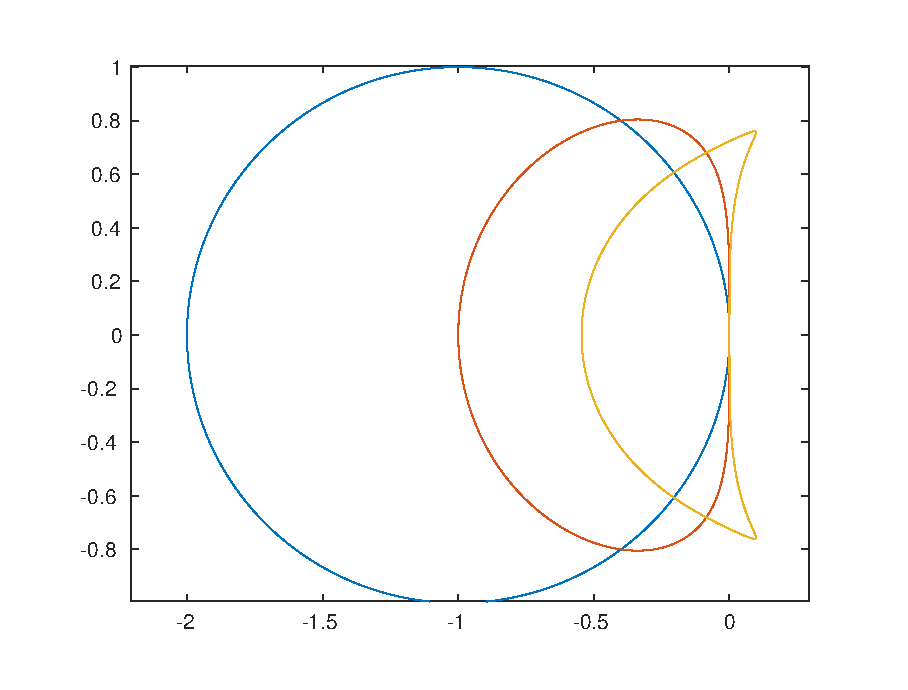
\includegraphics[width=0.9\linewidth]{figure/ex-11-138-1.eps}
        \caption*{Adams-Bashforth for $p=1,2,3$}
    \end{minipage}
    \hspace{1em}
    \begin{minipage}[t]{0.4\linewidth}
      \centering
      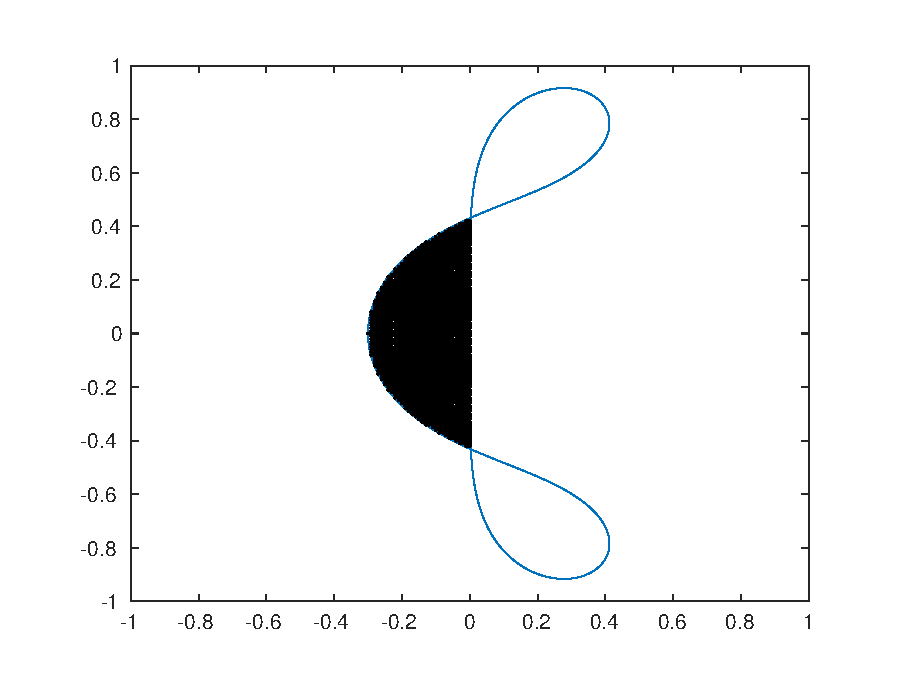
\includegraphics[width=0.9\linewidth]{figure/ex-11-138-2.eps}
      \caption*{Adams-Bashforth for $p=4$}
    \end{minipage}
    \begin{minipage}[t]{0.4\linewidth}
        \centering
        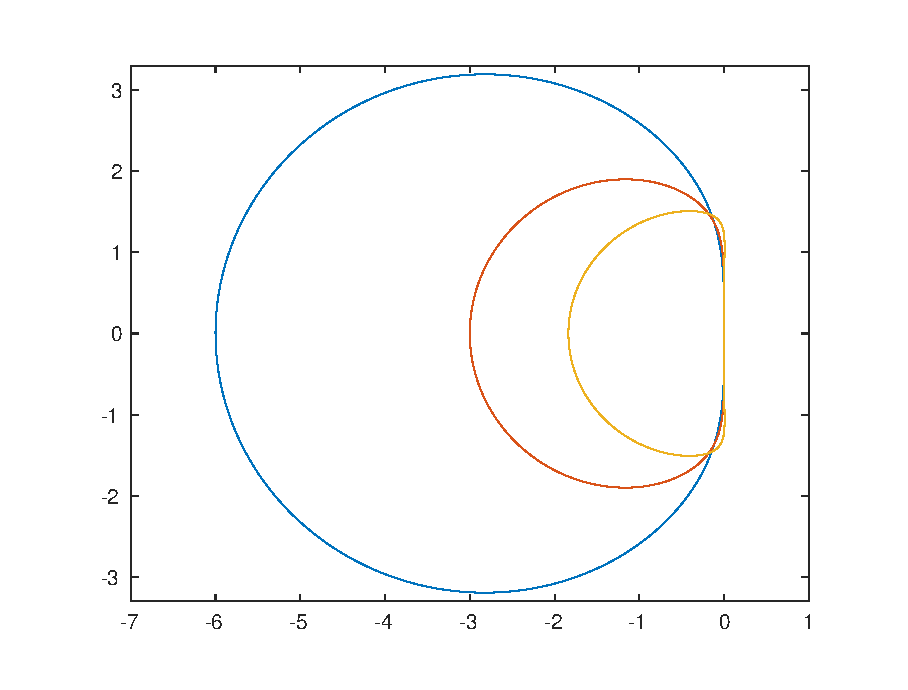
\includegraphics[width=0.9\linewidth]{figure/ex-11-139.eps}
        \caption*{Adams-Moulton for $p=3,4,5$}
    \end{minipage}
    \hspace{1em}
    \begin{minipage}[t]{0.4\linewidth}
        \centering
        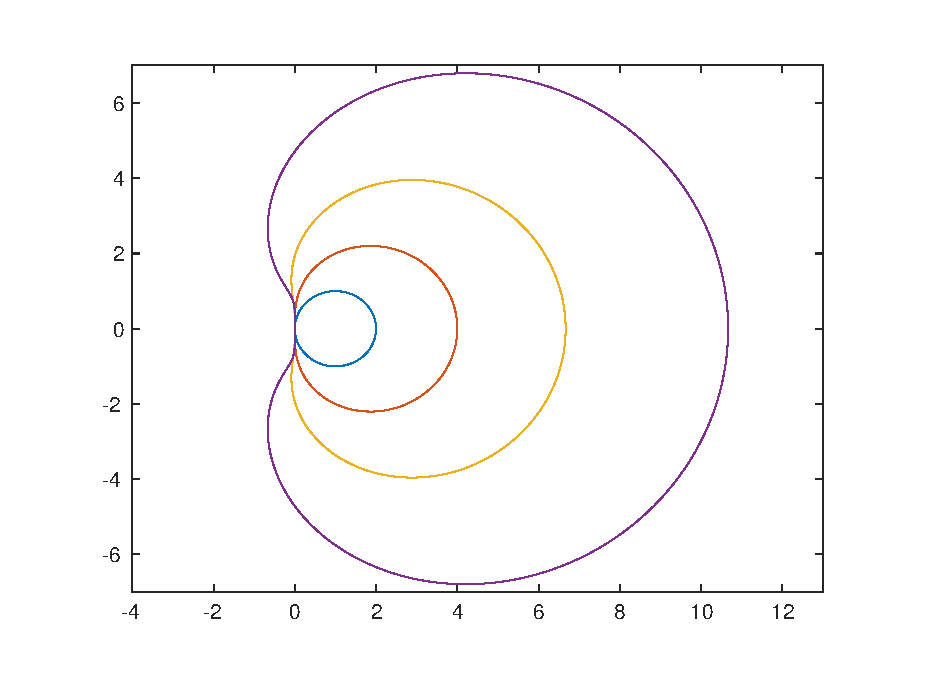
\includegraphics[width=0.9\linewidth]{figure/ex-11-140.eps}
        \caption*{BDF for $p=1,2,3,4$}
    \end{minipage}
\end{figure}

\textbf{The figures at Example 11.138 were reproduced by the following matlab code.}
\begin{lstlisting}
    B = [ 1, 0, 0, 0; -1/2, 3/2, 0, 0; 5/12, -4/3, 23/12, 0; -3/8, 37/24, -59/24, 55/24 ];
    % When producing the first figure, replace the 4:4 to 1:3.
    for s = 4:4
        b = B(s,:);
        rho = @(x)(x.^s-x.^(s-1));
        sigma = @(x)(b(1)+b(2)*x+b(3)*(x.^2)+b(4)*(x.^3));
        X = 0:0.01:2*pi;
        Y = rho(exp(1i*X))./sigma(exp(1i*X));
        plot(real(Y),imag(Y));
        xlim([-1,1]); ylim([-1,1]);
        hold on
    end
    % When producing the first figure, the codes below is not necessary.
    b = B(4,:);
    HX = zeros(201*201, 2); cnt = 0;
    for X = -1:0.01:1
        for Y = -1:0.01:1
            k = X + Y*1i;
            rho = [1, -1, 0, 0, 0];
            sigma = [0, b(4), b(3), b(2), b(1)];
            p = rho - k * sigma;
            if max(abs(roots(p)))<=1
                cnt = cnt + 1;
                HX(cnt,:) = [X, Y];
            end
        end
    end
    scatter(HX(:,1), HX(:,2), 2, "filled", 'k');
\end{lstlisting}

\textbf{The figure at Example 11.139 was reproduced by the following matlab code.}
\begin{lstlisting}
    B = [ -1/12, 2/3, 5/12, 0, 0; 1/24, -5/24, 19/24, 3/8, 0; -19/720, 53/360, -11/30, 
323/360, 251/720 ];
    for s = 1:3
        b = B(s,:);
        rho = @(x)(x.^(s+1)-x.^(s));
        sigma = @(x)(b(1)+b(2)*x+b(3)*(x.^2)+b(4)*(x.^3)+b(5)*(x.^4));
        X = 0:0.01:2*pi;
        Y = rho(exp(1i*X))./sigma(exp(1i*X));
        plot(real(Y),imag(Y));
        xlim([-7,1]); ylim([-3.3,3.3]);
        hold on
    end
\end{lstlisting}

\textbf{The figure at Example 11.140 was reproduced by the following matlab code.}
\begin{lstlisting}
    A = [ 1, -1, 1, 0, 0, 0; 1, -4/3, 1/3, 2/3, 0, 0; 1, -18/11, 9/11, -2/11, 6/11, 0; 
1, -48/25, 36/25, -16/25, 3/25, 12/25 ];
    for s = 1:4
        b = A(s,:);
        sigma = @(x)(b(2+s)*x.^s);
        X = exp(1i*(0:0.01:2*pi));
        rho = b(1)*(X.^s);
        for i = 2:s+1
            rho = rho + b(i)*(X.^(s+1-i));
        end
        Y = rho./sigma(X);
        plot(real(Y),imag(Y));
        xlim([-4,13]); ylim([-7,7]);
        hold on
    end
\end{lstlisting}

\end{document}

%%% Local Variables: 
%%% mode: latex
%%% TeX-master: t
%%% End: 
